\documentclass[border=3pt]{standalone}
% Preâmbulo compartilhado pelos diagramas TikZ da aula 10 (Localização de Markov e Gaussiana)
\usepackage[T1]{fontenc}
\usepackage[utf8]{inputenc}
\usepackage{lmodern}
\usepackage{amsmath}
\usepackage{xcolor}
\usepackage{tikz}
\usetikzlibrary{arrows.meta,angles,quotes,decorations.pathmorphing,calc,
                positioning,shapes.geometric,shapes.misc,backgrounds,fit,
                math}

% Paleta (mesma dos SVGs originais)
\definecolor{dblue}{HTML}{2A5B8C}
\definecolor{dorange}{HTML}{B3541E}
\definecolor{dgreen}{HTML}{4A7C59}
\definecolor{dred}{HTML}{9C4B4B}
\definecolor{dcream}{HTML}{F4F1EA}
\definecolor{dshade}{HTML}{DDD7C9}

% Função gaussiana (não normalizada por padrão de escala visual)
\pgfmathdeclarefunction{gauss}{3}{%
  \pgfmathparse{1/(#3*sqrt(2*pi))*exp(-((#1-#2)^2)/(2*#3^2))}%
}

% Estilos comuns (prefixo d... para não colidir com chaves internas do pgf)
\tikzset{
  >={Stealth[length=2mm]},
  dguide/.style={gray!55, dashed, line width=0.4pt},
  daxis/.style={gray!60, line width=0.7pt, ->},
  dbody/.style={fill=black!3, draw=black!80, line width=1pt},
  dacc/.style={draw=dblue, line width=1pt},
  dlbl/.style={black!55, font=\small},
  dsub/.style={black!45, font=\footnotesize},
  dstate/.style={circle, draw=black!80, fill=dcream, line width=1pt,
                 minimum size=17mm, font=\large, inner sep=1pt},
  dobs/.style={circle, draw=black!80, fill=dshade, line width=1pt,
               minimum size=14mm, font=\large, inner sep=1pt},
  dbox/.style={rounded corners=2pt, draw=black!80, fill=dcream, line width=1pt,
               align=center, inner sep=6pt},
  dop/.style={circle, draw=black!80, fill=white, line width=1pt,
              minimum size=6mm, inner sep=0pt, font=\small},
  dtrans/.style={->, dblue, line width=1pt},
  dmeas/.style={->, dorange, line width=1pt},
  dcurve/.style={line width=1pt, dblue},
  dcurveb/.style={line width=1.4pt, dorange},
}

\usetikzlibrary{shapes.callouts}
\begin{document}
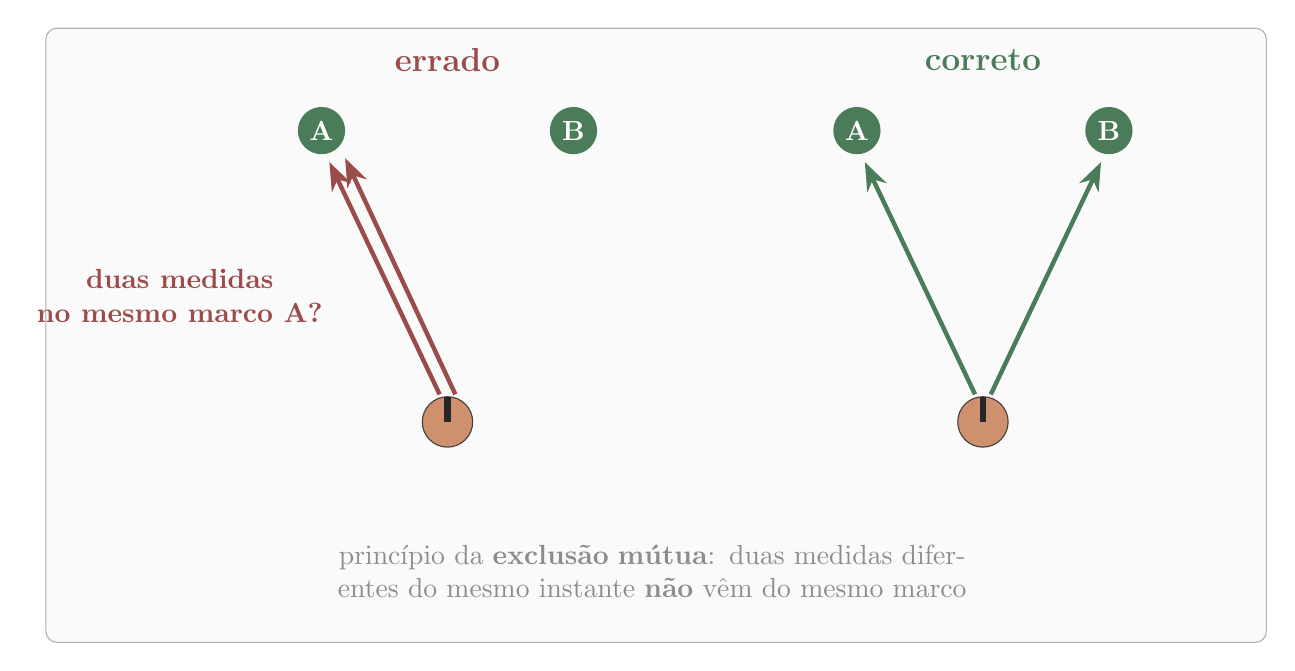
\begin{tikzpicture}[x=1cm,y=1cm,bal/.style={rectangle callout, rounded corners=7pt, draw=black!75, fill=white, line width=1pt, align=center, font=\normalsize, inner sep=5pt}]
\draw[black!30, fill=black!2, rounded corners=4pt] (-0.5,-2.2) rectangle (15,5.6);
\fill[dgreen] (3.0,4.3) circle (0.3); \node[white, font=\normalsize\bfseries] at (3.0,4.3) {A}; \fill[dgreen] (6.2,4.3) circle (0.3); \node[white, font=\normalsize\bfseries] at (6.2,4.3) {B};
\fill[dorange!65, draw=black!75] (4.6,0.6) circle (0.32); \draw[black!85, line width=2.4pt] (4.6,0.6) -- (4.6,0.92);
\draw[dred, line width=1.6pt, -{Stealth}] (4.5,0.95) -- (3.1,3.9); \draw[dred, line width=1.6pt, -{Stealth}] (4.7,0.95) -- (3.3,3.95);
\node[dred, font=\normalsize\bfseries, align=center] at (1.2,2.2) {duas medidas\\ no mesmo marco A?};
\node[font=\bfseries\large, dred] at (4.6,5.2) {errado};
\begin{scope}[shift={(8.8,0)}]
\fill[dgreen] (1.0,4.3) circle (0.3); \node[white, font=\normalsize\bfseries] at (1.0,4.3) {A}; \fill[dgreen] (4.2,4.3) circle (0.3); \node[white, font=\normalsize\bfseries] at (4.2,4.3) {B};
\fill[dorange!65, draw=black!75] (2.6,0.6) circle (0.32); \draw[black!85, line width=2.4pt] (2.6,0.6) -- (2.6,0.92);
\draw[dgreen, line width=1.6pt, -{Stealth}] (2.5,0.95) -- (1.1,3.9); \draw[dgreen, line width=1.6pt, -{Stealth}] (2.7,0.95) -- (4.1,3.9);
\node[font=\bfseries\large, dgreen] at (2.6,5.2) {correto};
\end{scope}
\node[dsub, font=\normalsize, align=center, text width=13cm] at (7.2,-1.3) {princípio da \textbf{exclusão mútua}: duas medidas diferentes do mesmo instante \textbf{não} vêm do mesmo marco};
\end{tikzpicture}
\end{document}
